% Author: Dominik Harmim <harmim6@gmail.com>


\documentclass[10pt, xcolor=pdflatex, hyperref={unicode}, aspectratio=169]{beamer}


\usepackage{newcent}
\usepackage[utf8]{inputenc}
\usepackage[british]{babel}
\usepackage[T1]{fontenc}
\usepackage{xcolor}
\usepackage{booktabs}

\definecolor{thread1}{HTML}{DE5C82}
\definecolor{thread2}{HTML}{009999}
\definecolor{darkgreen}{RGB}{53, 142, 5}

\newcommand\tab[1][1cm]{\hspace*{#1}}

% Setting of a path to the pictures.
\graphicspath{{img/}}


%%%%%%%%%%%%%%%%%%%%%%%%%%%%%%%%%%%%%%%%%%%%%%%%%%%%%%%%%%%%%%%%%%%%%%%%%%%%%%%%


\usetheme{FIT}

\title[Static Deadlock Detection in Low-Level C~Code]{Static Deadlock Detection in Low-Level C~Code}
\subtitle{\texorpdfstring{Eurocast'22\,---\,Model-Based System Design, Verification, and Simulation Workshop}{Eurocast'22 - Model-Based System Design, Verification, and Simulation Workshop}}

\author{\texorpdfstring{%
    Dominik Harmim \\
    \footnotesize{Vladimír Marcin, Lucie Svobodová, Tomáš Vojnar}%
}{Dominik Harmim; Vladimír Marcin, Lucie Svobodová, Tomáš Vojnar}}

\institute{%
    iharmim@fit.vut.cz \\
    Czech Republic, Brno University of Technology, Faculty of Information Technology, VeriFIT%
}

\subject{Eurocast'22 Presentation}

\date{\today}


%%%%%%%%%%%%%%%%%%%%%%%%%%%%%%%%%%%%%%%%%%%%%%%%%%%%%%%%%%%%%%%%%%%%%%%%%%%%%%%%


\begin{document}


%%%%%%%%%%%%%%%%%%%%%%%%%%%%%%%%%%%%%%%%%%%%%%%%%%%%%%%%%%%%%%%%%%%%%%%%%%%%%%%%


\section{Title Slide}
\frame[plain]{\titlepage}


%%%%%%%%%%%%%%%%%%%%%%%%%%%%%%%%%%%%%%%%%%%%%%%%%%%%%%%%%%%%%%%%%%%%%%%%%%%%%%%%


\section{Facebook Infer}
\begin{frame}{Facebook \textsc{Infer}}
    \begin{columns}
        \begin{column}{1 \linewidth}
            \begin{itemize}
                \item Open-source \alert{static analysis framework} for \emph{interprocedural analyses}.
                    \medskip
                    \begin{itemize}\setlength\itemsep{.8em}
                        \item Based on \alert{abstract interpretation}.

                        \item Checks, e.g., for buffer overflows, null-dereferencing, or memory leaks.
                    \end{itemize}
            \end{itemize}
        \end{column}
        \hfill
    \end{columns}

    \medskip

    \begin{columns}
        \begin{column}{.55 \linewidth}
            \begin{itemize}\setlength\itemsep{2em}
                \item Highly \alert{scalable}.
                    \medskip
                    \begin{itemize}\setlength\itemsep{.8em}
                        \item \emph{Compositional} and \emph{incremental} analysis.

                        \item Computes function \emph{summaries} \alert{bottom-up} on call-trees.
                    \end{itemize}

                \item Supports C, C++, Java, Obj-C, C\#.
            \end{itemize}
        \end{column}

        \begin{column}{.45 \linewidth}
            \centering
            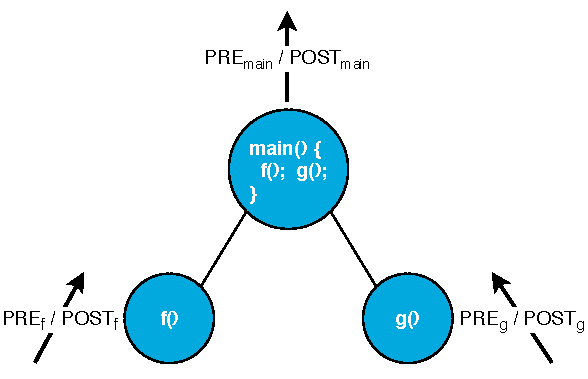
\includegraphics[width=1 \linewidth]{infer.pdf}
        \end{column}
    \end{columns}
\end{frame}


%%%%%%%%%%%%%%%%%%%%%%%%%%%%%%%%%%%%%%%%%%%%%%%%%%%%%%%%%%%%%%%%%%%%%%%%%%%%%%%%


\section{L2D2: A~Low-Level Deadlock Detector}
\begin{frame}{\textsc{L2D2}: A~Low-Level Deadlock Detector}
    \begin{columns}
        \begin{column}{.6 \linewidth}
            \begin{itemize}\setlength\itemsep{1em}
                \item \alert{Deadlocks}: among the best-known concurrency errors, caused by a~wrong \\ order of locking.

                \item \textsc{\alert{L2D2}}: a~novel deadlock analyser in \textsc{Infer}.

                \item For \emph{low-level, unstructured, C-style locking}.

                \item Based on computing so-called \alert{locksets}.

                \item \emph{Lockset analysis}:
                    \vspace{.5em}
                    \begin{itemize}
                        \item[] \alert{\textbf{\{\ \}}} $ \rightarrow $ \texttt{lock(\alert{\textbf{L}})} $ \rightarrow $ \alert{\textbf{\{\,\texttt{L}\,\}}} $ \rightarrow $ \texttt{unlock(\alert{\textbf{L}})} $ \rightarrow $ \alert{\textbf{\{\ \}}}
                    \end{itemize}
            \end{itemize}
        \end{column}

        \begin{column}{.4 \linewidth}
            \hspace*{-2.5em}
            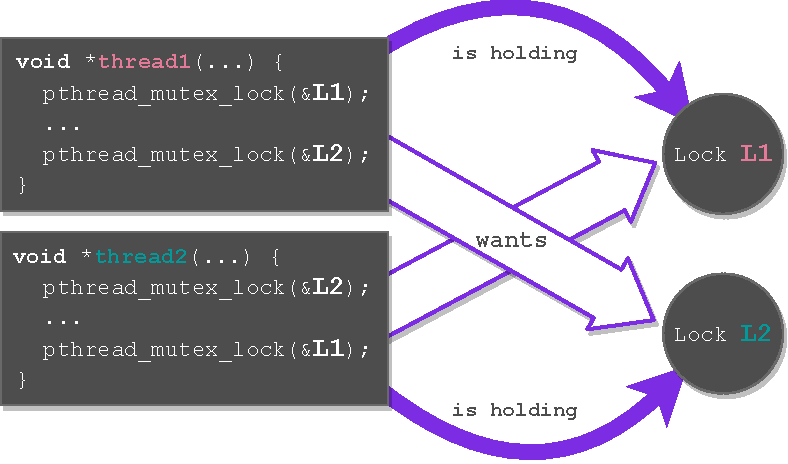
\includegraphics[scale=.5]{deadlock.pdf}
        \end{column}
    \end{columns}
\end{frame}


%%%%%%%%%%%%%%%%%%%%%%%%%%%%%%%%%%%%%%%%%%%%%%%%%%%%%%%%%%%%%%%%%%%%%%%%%%%%%%%%


\section{Related Work}
\begin{frame}{Related Work}
    \begin{itemize}\setlength\itemsep{2em}
        \item \textbf{Dynamic deadlock analysers and testing:}
            \medskip
            \begin{itemize}\setlength\itemsep{.5em}
                \item \alert{Test coverage} is \emph{insufficient} (can not be sound).

                \item It may be improved by, e.g., \emph{systematic testing}, \emph{noise-based testing}, or \alert{extrapolation} (\textsc{GoodLock}, \textsc{AirLock}\,---\,ICSE'20).

                \item Requires \emph{input data}, \alert{does not scale enough}, and not have to be even complete.
            \end{itemize}

        \item \textbf{Static deadlock analysers:}
            \medskip
            \begin{itemize}\setlength\itemsep{.5em}
                \item \textsc{RacerX}\,---\,similar to \textsc{L2D2} but it is \emph{context-sensitive} (thus \alert{not scale so well}).

                \item \textsc{Starvation}\,---\,\alert{compositional} analyser implemented in \textsc{Infer} (ASE'21).
                    \begin{itemize}
                        \item Limited to \emph{high-level Java and C++ programs} only.
                    \end{itemize}

                \item Often not sound nor complete in practise (\emph{heuristics needed}).
            \end{itemize}

        \item \textbf{There is \alert{no} \emph{compositional} static deadlock analyser for \emph{low-level code}.}
    \end{itemize}
\end{frame}


%%%%%%%%%%%%%%%%%%%%%%%%%%%%%%%%%%%%%%%%%%%%%%%%%%%%%%%%%%%%%%%%%%%%%%%%%%%%%%%%


\section{Function Summaries - Basic Idea}
\begin{frame}{Function Summaries\,---\,Basic Idea}
    \begin{center}
        \large
        \{\,($ Locked $, $ Unlocked $)\,\} \\
        \textbf{\texttt{foo()}} \\
        \{\,($ Lockset $, $ Unlockset $, $ Dependencies $)\,\}
    \end{center}

    \begin{itemize}\setlength\itemsep{1.5em}
        \item \textbf{Pre-Condition:}
            \vspace{.3em}
            \begin{itemize}\setlength\itemsep{.5em}
                \item \alert{$ Locked $}: locks that should be \emph{locked} before calling the function.
                    \begin{itemize}
                        \item The function starts by \emph{unlocking} the given lock.
                    \end{itemize}

                \item \alert{$ Unlocked $}: locks that should be \emph{unlocked} before calling the function.
                    \begin{itemize}
                        \item The function starts by \emph{locking} the given lock.
                    \end{itemize}
            \end{itemize}

        \item \textbf{Post-Condition:}
            \vspace{.3em}
            \begin{itemize}\setlength\itemsep{.5em}
                \item \alert{$ Lockset $}: locks that \emph{may be locked} at exit.

                \item \alert{$ Unlockset $}: locks that \emph{may be unlocked} at exit.

                \item \alert{$ Dependencies $}: record that some lock got \emph{locked} while another lock was \emph{still held},
                    \begin{itemize}
                        \item i.e., the \emph{order of locking}.
                    \end{itemize}
            \end{itemize}
    \end{itemize}
\end{frame}


%%%%%%%%%%%%%%%%%%%%%%%%%%%%%%%%%%%%%%%%%%%%%%%%%%%%%%%%%%%%%%%%%%%%%%%%%%%%%%%%


\section{Function Summaries - An Example}
\begin{frame}{Function Summaries\,---\,An Example}
    \centering
    \only<1>{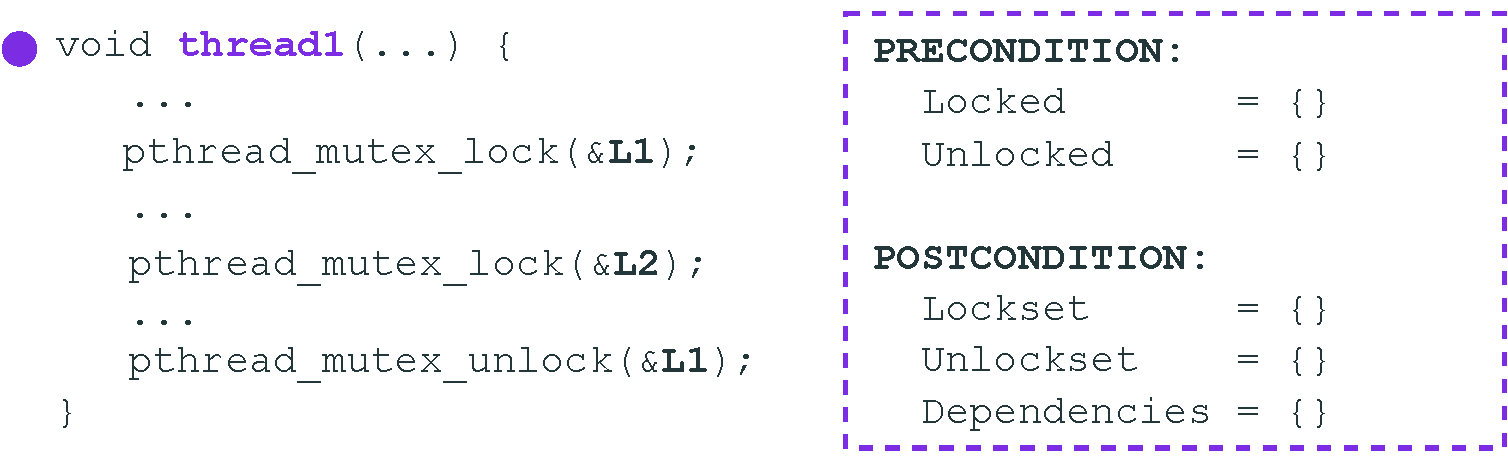
\includegraphics[width=1 \linewidth]{basSummL2D2-1.pdf}}
    \only<2>{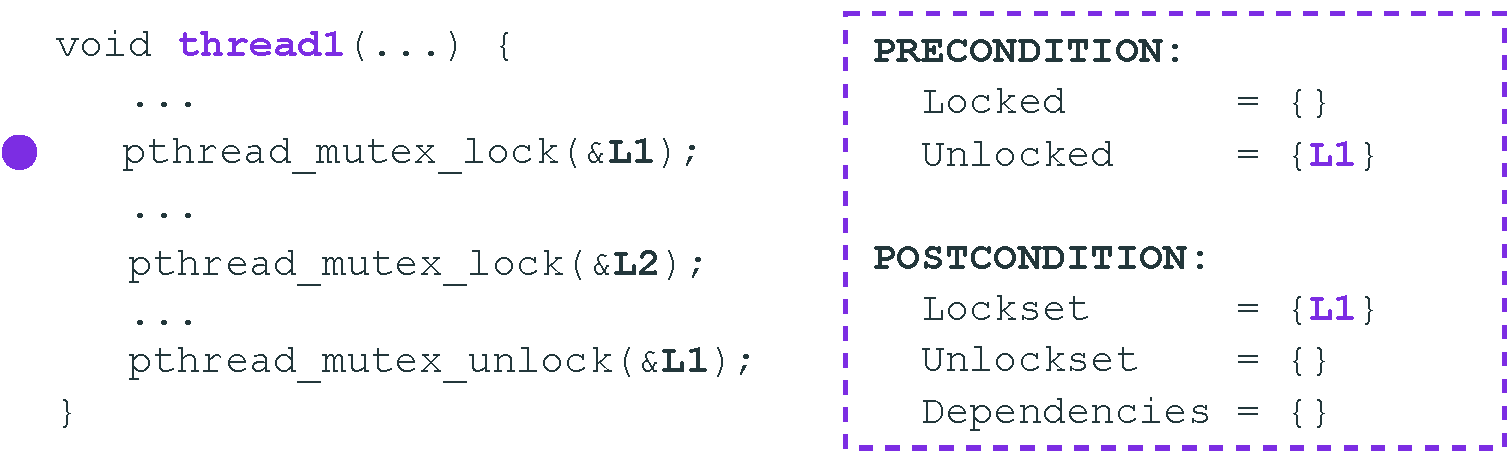
\includegraphics[width=1 \linewidth]{basSummL2D2-2.pdf}}
    \only<3>{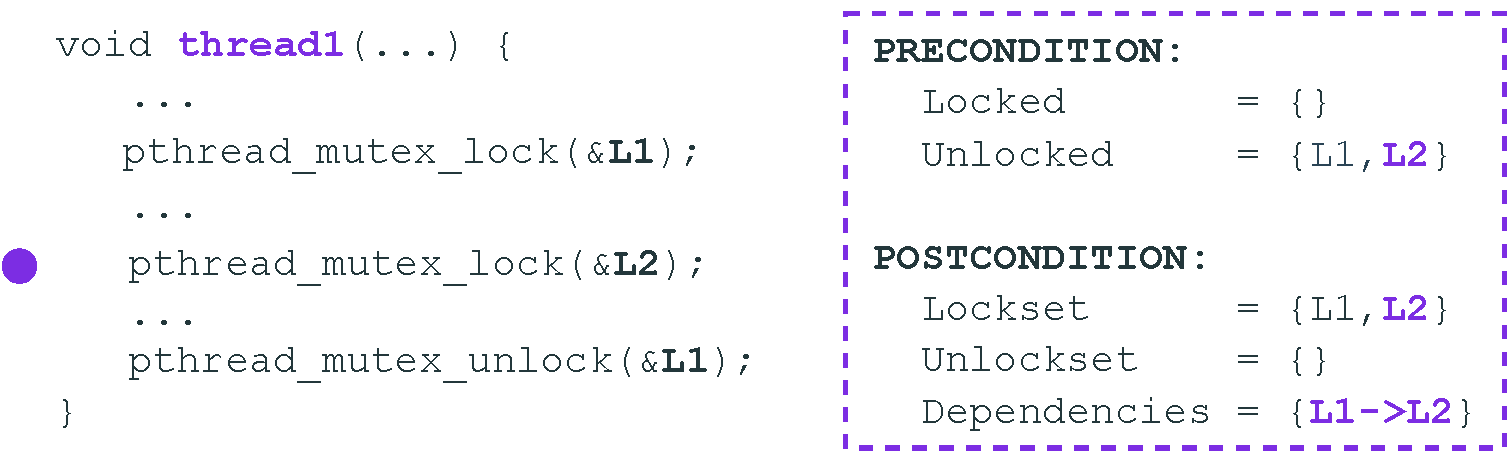
\includegraphics[width=1 \linewidth]{basSummL2D2-3.pdf}}
    \only<4>{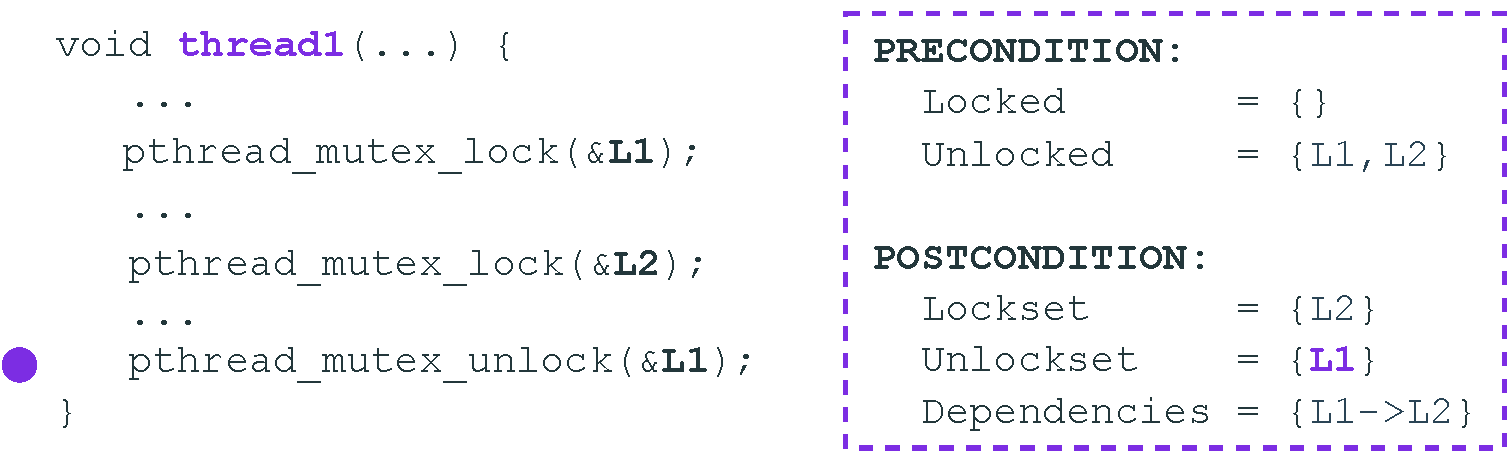
\includegraphics[width=1 \linewidth]{basSummL2D2-4.pdf}}
    \only<5>{\vspace{-.8em}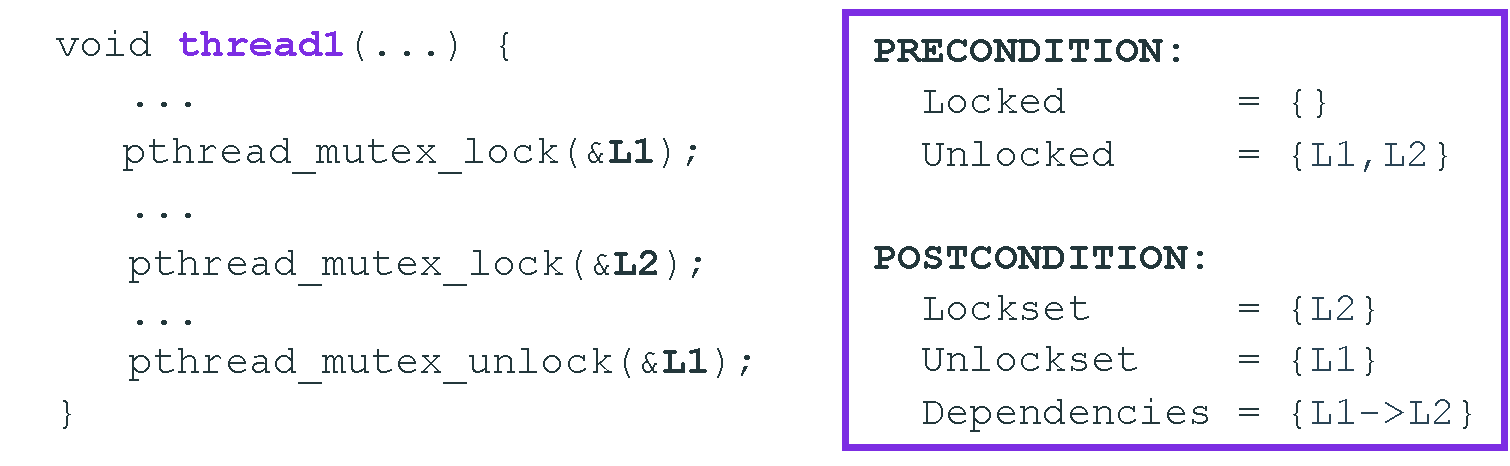
\includegraphics[width=1 \linewidth]{basSummL2D2-5.pdf}}
\end{frame}


%%%%%%%%%%%%%%%%%%%%%%%%%%%%%%%%%%%%%%%%%%%%%%%%%%%%%%%%%%%%%%%%%%%%%%%%%%%%%%%%


\section{Function Summaries - Tricky Cases}
\begin{frame}{Function Summaries\,---\,Tricky Cases}
    \begin{columns}
        \begin{column}{.75 \linewidth}
            \begin{enumerate}
                \item Locks both \emph{acquired} and \emph{released} in a~function:
                    \vspace{.5em}
                    \begin{itemize}\setlength\itemsep{.5em}
                        \item Can be deduced from $ Unlockset $ and $ Unlocked $.

                        \item $ Unlockset $/$ Unlocked $ are erased in some situations.

                        \item \alert{$ WereLocked $}: all locks at least once locked (never erased).
                            \begin{itemize}
                                \item For example: $ \mathtt{L} \in WereLocked $ for \texttt{f()}.
                            \end{itemize}
                    \end{itemize}

                \vspace{2em}

                \item \emph{Locking interleaved with unlocking} across functions:
                \vspace{.5em}
                \begin{itemize}\setlength\itemsep{.5em}
                    \item Leads to a~false dependence.

                    \item \alert{$ Order $}: records unlock operations preceding lock operations.
                        \begin{itemize}
                            \item For example: $ \mathtt{L1} \rightarrow \mathtt{L2} \in Order $ for \texttt{h()}.
                        \end{itemize}
                \end{itemize}
            \end{enumerate}
        \end{column}

        \begin{column}{.25 \linewidth}
            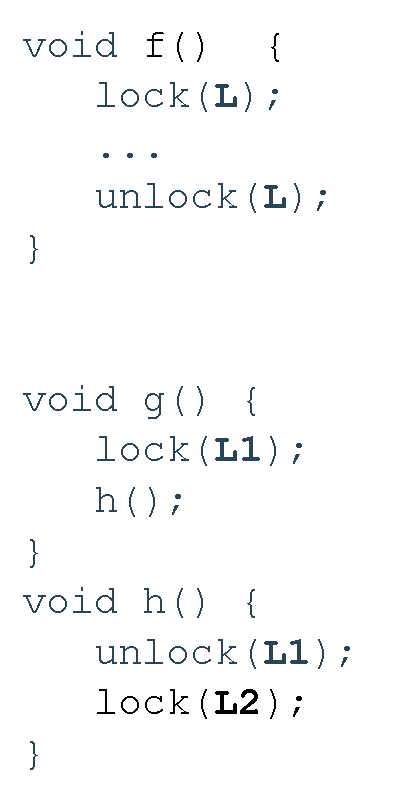
\includegraphics[scale=.5]{extSummL2D2.pdf}
        \end{column}
    \end{columns}
\end{frame}


%%%%%%%%%%%%%%%%%%%%%%%%%%%%%%%%%%%%%%%%%%%%%%%%%%%%%%%%%%%%%%%%%%%%%%%%%%%%%%%%


\section{Extended Summaries - An Example}
\begin{frame}{Extended Summaries\,---\,An Example}
    \centering
    \only<1>{\vspace{1.6em}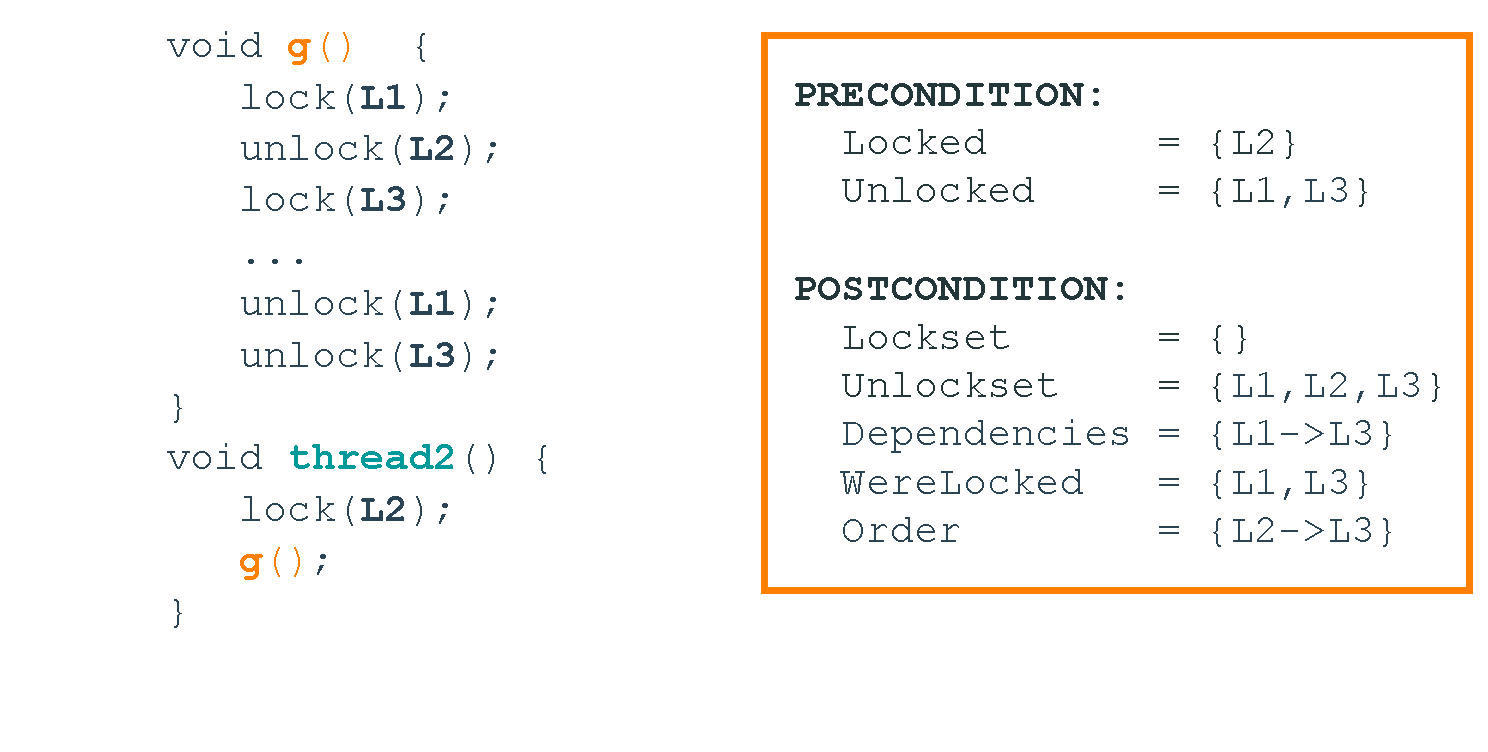
\includegraphics[width=1 \linewidth]{extSummL2D2-1.pdf}}
    \only<2>{\vspace{1.6em}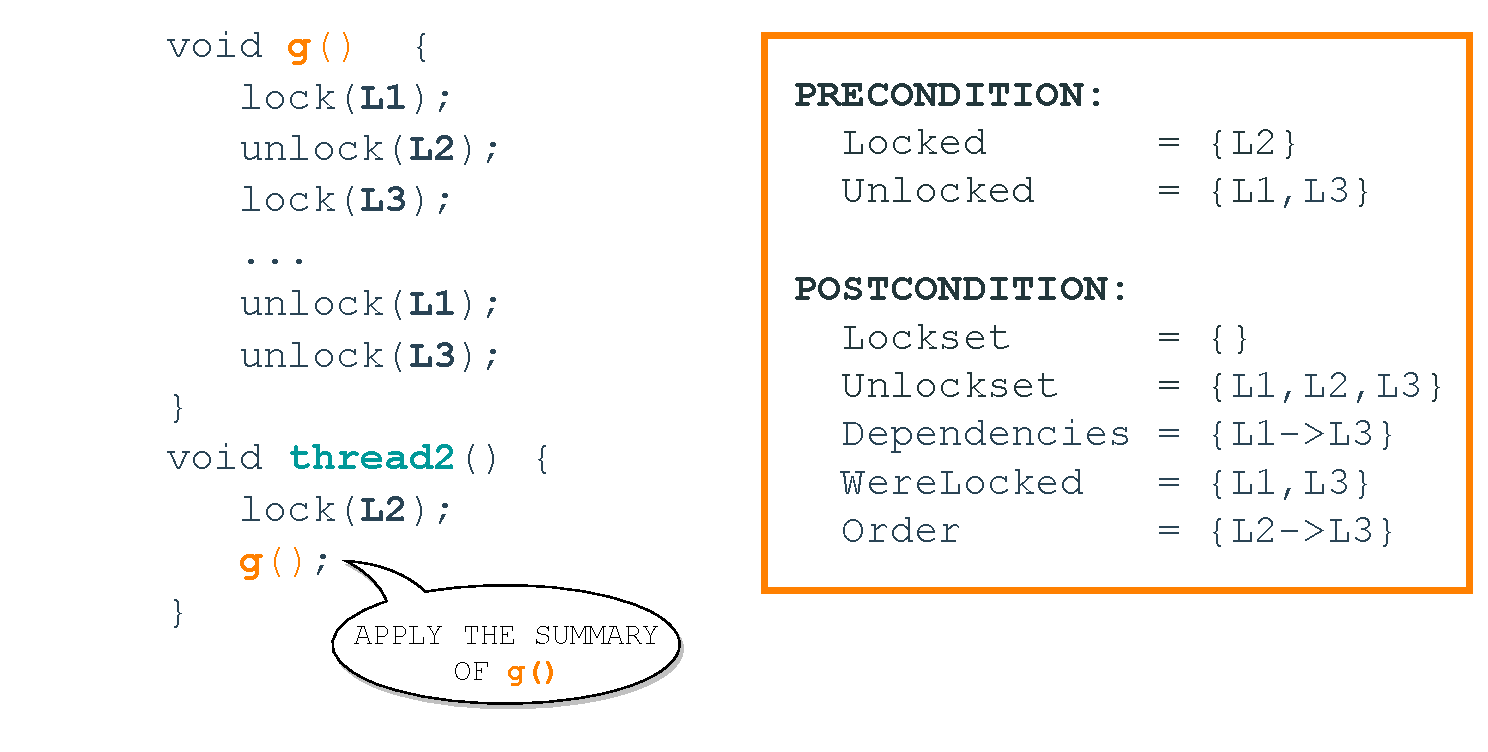
\includegraphics[width=1 \linewidth]{extSummL2D2-2.pdf}}
    \only<3>{\vspace{1.6em}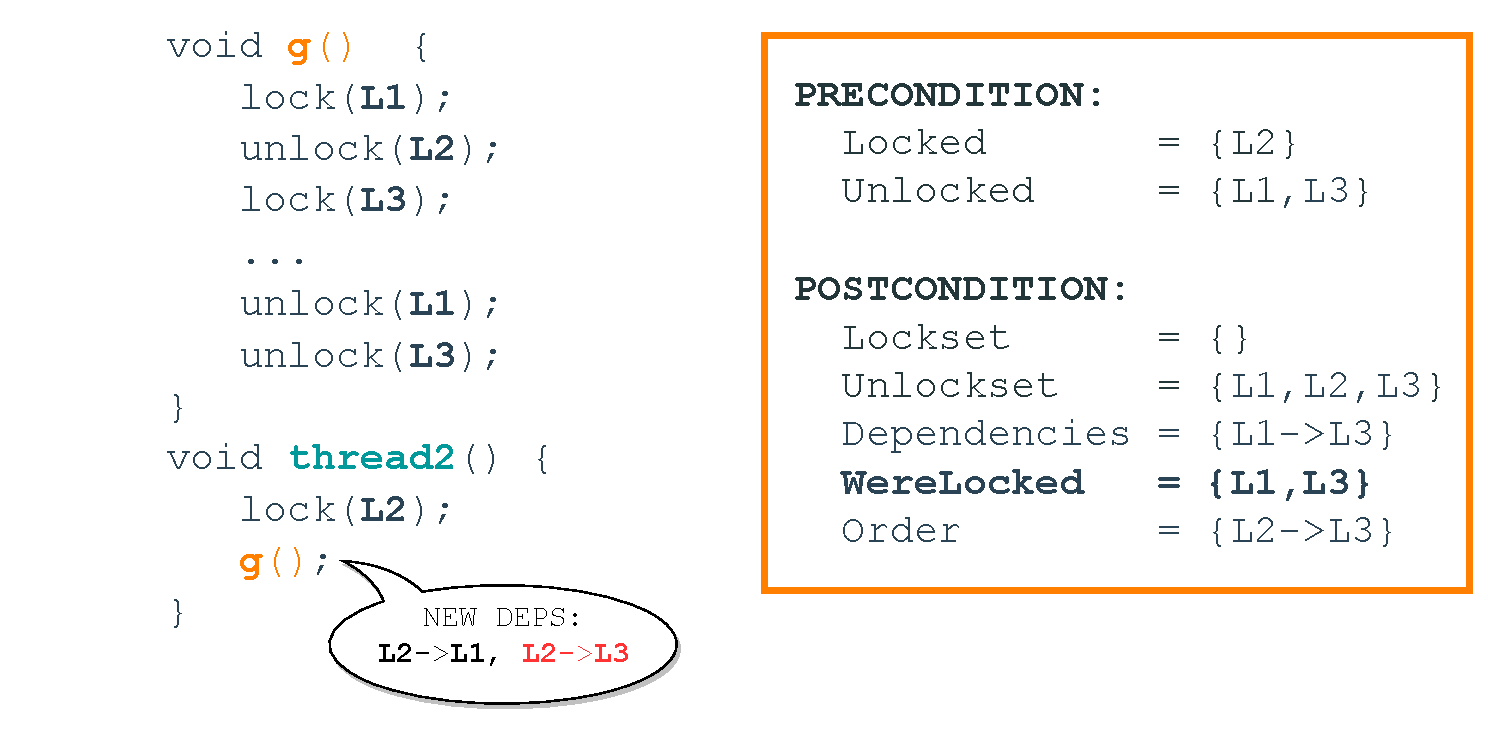
\includegraphics[width=1 \linewidth]{extSummL2D2-3.pdf}}
    \only<4>{\vspace{1.5em}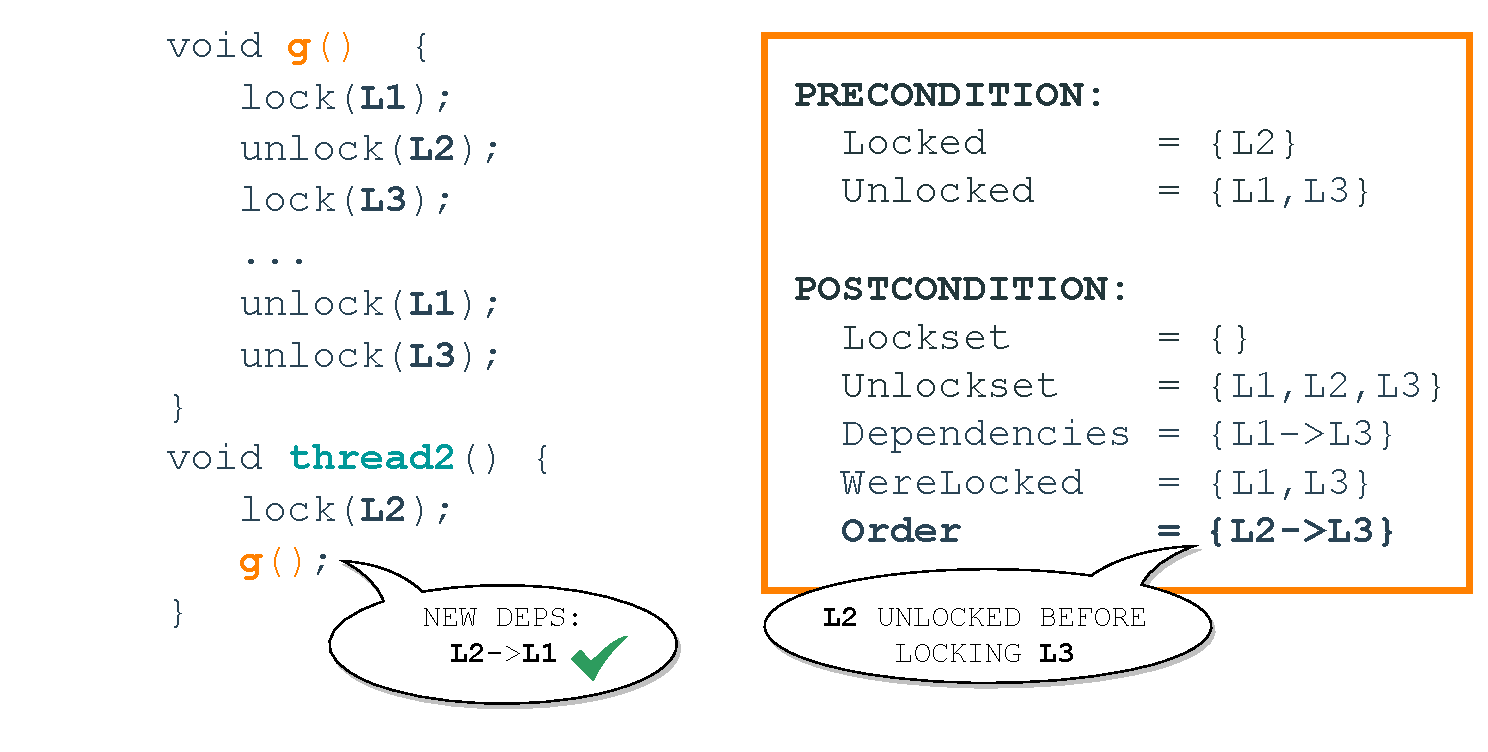
\includegraphics[width=1 \linewidth]{extSummL2D2-4.pdf}}
\end{frame}


%%%%%%%%%%%%%%%%%%%%%%%%%%%%%%%%%%%%%%%%%%%%%%%%%%%%%%%%%%%%%%%%%%%%%%%%%%%%%%%%


\section{Deadlock Detection}
\begin{frame}{Deadlock Detection}
    \begin{itemize}\setlength\itemsep{3em}
        \item \textbf{Pass~1:} \emph{summary construction}: \\
            \vspace{.5em}
            \begin{center}
                \{\,($ Locked $, $ Unlocked $)\,\} \\
                \textbf{\texttt{foo()}} \\
                \{\,($ Lockset $, $ Unlockset $, \alert{$ Dependencies $}, $ WereLocked $, $ Order $)\,\}
            \end{center}

        \item \textbf{Pass~2:} compute the \emph{transitive closure} of \alert{$ Dependencies $} \& flag cycles: \\
            \vspace{.5em}

            \textcolor{thread1}{\texttt{lock(L1);}\tab\tab[1.2cm] \textcolor{thread2}{\texttt{lock(L2);}}}

            \textcolor{thread2}{\texttt{lock(L2);}\tab\tab[1.2cm] \textcolor{thread1}{\texttt{lock(L1);}}}

            \vspace{1em}

            \texttt{\textbf{\textcolor{thread1}{L1}} $ \rightarrow $ \textbf{\textcolor{thread2}{L2}} $ \rightarrow $ \textbf{\textcolor{thread1}{L1}} $ \Rightarrow $} \textbf{\alert{Deadlock}}
    \end{itemize}
\end{frame}


%%%%%%%%%%%%%%%%%%%%%%%%%%%%%%%%%%%%%%%%%%%%%%%%%%%%%%%%%%%%%%%%%%%%%%%%%%%%%%%%


\section{Extensions and Heuristics}
\begin{frame}{Extensions and Heuristics}
    \begin{itemize}\setlength\itemsep{3em}
        \item Optional \emph{reduction of potential false deadlocks} by erasing the locksets upon \alert{detection of double (un)locking}.

        \item Detecting \alert{gate locks} and ignoring false deadlocks guarded by them.

        \item \emph{Approximating lock objects} using \alert{syntactic access paths},
            \medskip
            \begin{itemize}\setlength\itemsep{.5em}
                \item i.e., a~representation of \emph{heap locations} via the paths used to access them.
            \end{itemize}
    \end{itemize}
\end{frame}


%%%%%%%%%%%%%%%%%%%%%%%%%%%%%%%%%%%%%%%%%%%%%%%%%%%%%%%%%%%%%%%%%%%%%%%%%%%%%%%%


\section{Experimental Evaluation}
\begin{frame}{Experimental Evaluation}
    \normalsize{On the benchmarks used for evaluating the \emph{\textsc{CProver} deadlock checker} from:}
    \begin{thebibliography}{1}
        \normalsize
        \bibitem[kroening]{kroening}
        \textsc{Kroening, D.; Poetzl, D.; Schrammel, P.}; et al.: \textit{Sound Static Deadlock Analysis for C/Pthreads}. ASE 2016.
    \end{thebibliography}

    \bigskip

    \begin{columns}
        \begin{column}{.5 \linewidth}
            \begin{itemize}\setlength\itemsep{.5em}
                \item \alert{11.4\,MLOC} from \emph{Debian GNU/Linux}.

                \item \alert{100\,\% deadlock detection} rate.

                \item Roughly \alert{4\,\% false positives} rate.

                \item Less than \alert{1\,\%} of the time of \textsc{CProver}.
            \end{itemize}
        \end{column}

        \begin{column}{.5 \linewidth}
            \begin{tabular}{lrr}
                & \textsc{\alert{\textbf{L2D2}}} & \textsc{CProver} \\ \midrule

                Deadlocks & \textcolor{darkgreen}{8} & \textcolor{darkgreen}{8} \\

                False Positives & \textcolor{red}{39} & \textcolor{red}{114} \\

                No Deadlocks & \textcolor{darkgreen}{877} & \textcolor{darkgreen}{292} \\

                Failed Cases & \textcolor{red}{80} & \textcolor{red}{588} \\ \bottomrule \\[-1em]

                \textbf{Total} & 1\,002 & 1\,002
            \end{tabular}
        \end{column}
    \end{columns}
\end{frame}


%%%%%%%%%%%%%%%%%%%%%%%%%%%%%%%%%%%%%%%%%%%%%%%%%%%%%%%%%%%%%%%%%%%%%%%%%%%%%%%%


\end{document}
